To simplify searching a large database such as the human genome there are two major categories: seed-and-extend heuristic methods and suffix-array mapping methods. The \emph{seed-and-extend} heuristic is developed based on the observation that for a correct mapping, the short query read and its corresponding reference fragment, which is the piece of the reference genome that the query read should map to, must share some brief regions (usually 10-100 base-pair-long) of exact or inexact matches. These shorter shared regions, which indicate high similarity between the query read and the reference fragment, are called seeds. By identifying the seeds of a query read, the mapper narrows down the searching range from the whole genome to only the neighborhood region of each seed. Seeds are generated by preprocessing the reference genome and storing the locations of their occurrences in the reference genome in a separate data structure. During mapping, a seed-and-extend mapper first analyzes the query read to identify the seeds. Then, the mapper tries to extend the read at each of the seed locations via dynamic programming algorithms such as the Smith-Waterman \citep{smith1981identification} or Neddleman-Wunsch \citep{needleman} algorithm.

During few years ago several mappers have been developed. These mappers basically work base on two approaches: 1)hash table based, using in seed and extend approach and 2) suffixarray and genome compression based mappers that utilize the Burrows-Wheeler Transform and the FerraginaManzini index (BWT-FM).  mrFAST/mrsFASt \cite{mrfast}\cite{mrsfast}, drFAST\cite{drfast} and RazerS\cite{razers} are examples of hash table based method and mappers such as BWA\cite{bwa} and Bowtie\cite{bowtie} are examples for BWT-FM approach. 

To compare these  methods with each other there are three metrics: \emph{speed (or performance)}, \emph{sensitivity} and \emph{comprehensiveness}. Essantially, hash table based mappers are more sensitive in compare with suffix-array based mappers but in cost of speed and performance. In addition, they are more comprehensive and more robust to sequence errors and genomic diversity.

The relatively slow speed of hash table based mappers is due to their high sensitivity and comprehensiveness. Such mappers first index fixed-length seeds (also called \emph{k-mers}), typically 10-13 base-pair-long DNA fragments from the reference genome, into a hash table or a similar data structure. Next, they divide each query read into smaller fixed length seeds to query the hash table for their associated seed locations. Finally, they try to extend the read at each of the seed locations by aligning the read to the reference fragment at the seed location via dynamic programming algorithms such as Needleman-Wunsch \cite{needleman} and SmithWaterman \cite{smith1981identification}, or \emph{simple Hamming distance} calculation for greater speed at the cost of missing potential mappings that contain insertions/deletions (indels).

According to \cite{fasthash} using data provided by NGS platform shows most of the \textit{locations} fail to provide correct alignments.This is because the size of the k-mers that form the hash table’s indices are typically very short. Eeven though in mrsFAST-ultra\cite{mrsfastultra} for indexing part author is using a variation of this method but the problem is still consist. The problem is these short k-mers appear in the reference genome much more frequently than the undivided, hundreds of base-pair-long query read. As a result, only a few of the locations of a k-mer, if any, provide correct alignments. In other words, Read mappers identify locations within a reference genome where the read and the reference match within a user-defined error (i.e., insertions, deletions, or substitutions) threshold, e. In practice, e is usually $5\%$ of the read length, but most aligners can be configured to return only the best mapping (the mapping with the fewest errors). As seen in Figure 1 \cite{shd}, most potential location mappings tested by seed-and-extend based mappers are incorrect (having more errors than allowed); in fact, when e = $5\%$ of the read length, more than $98\%$ of mappings are incorrect. Since alignment is the primary computationally intensive task performed by seed-and-extend based read mappers \cite{fasthash}, it is crucial that incorrect mappings be rejected efficiently. 
  
\begin{figure}
    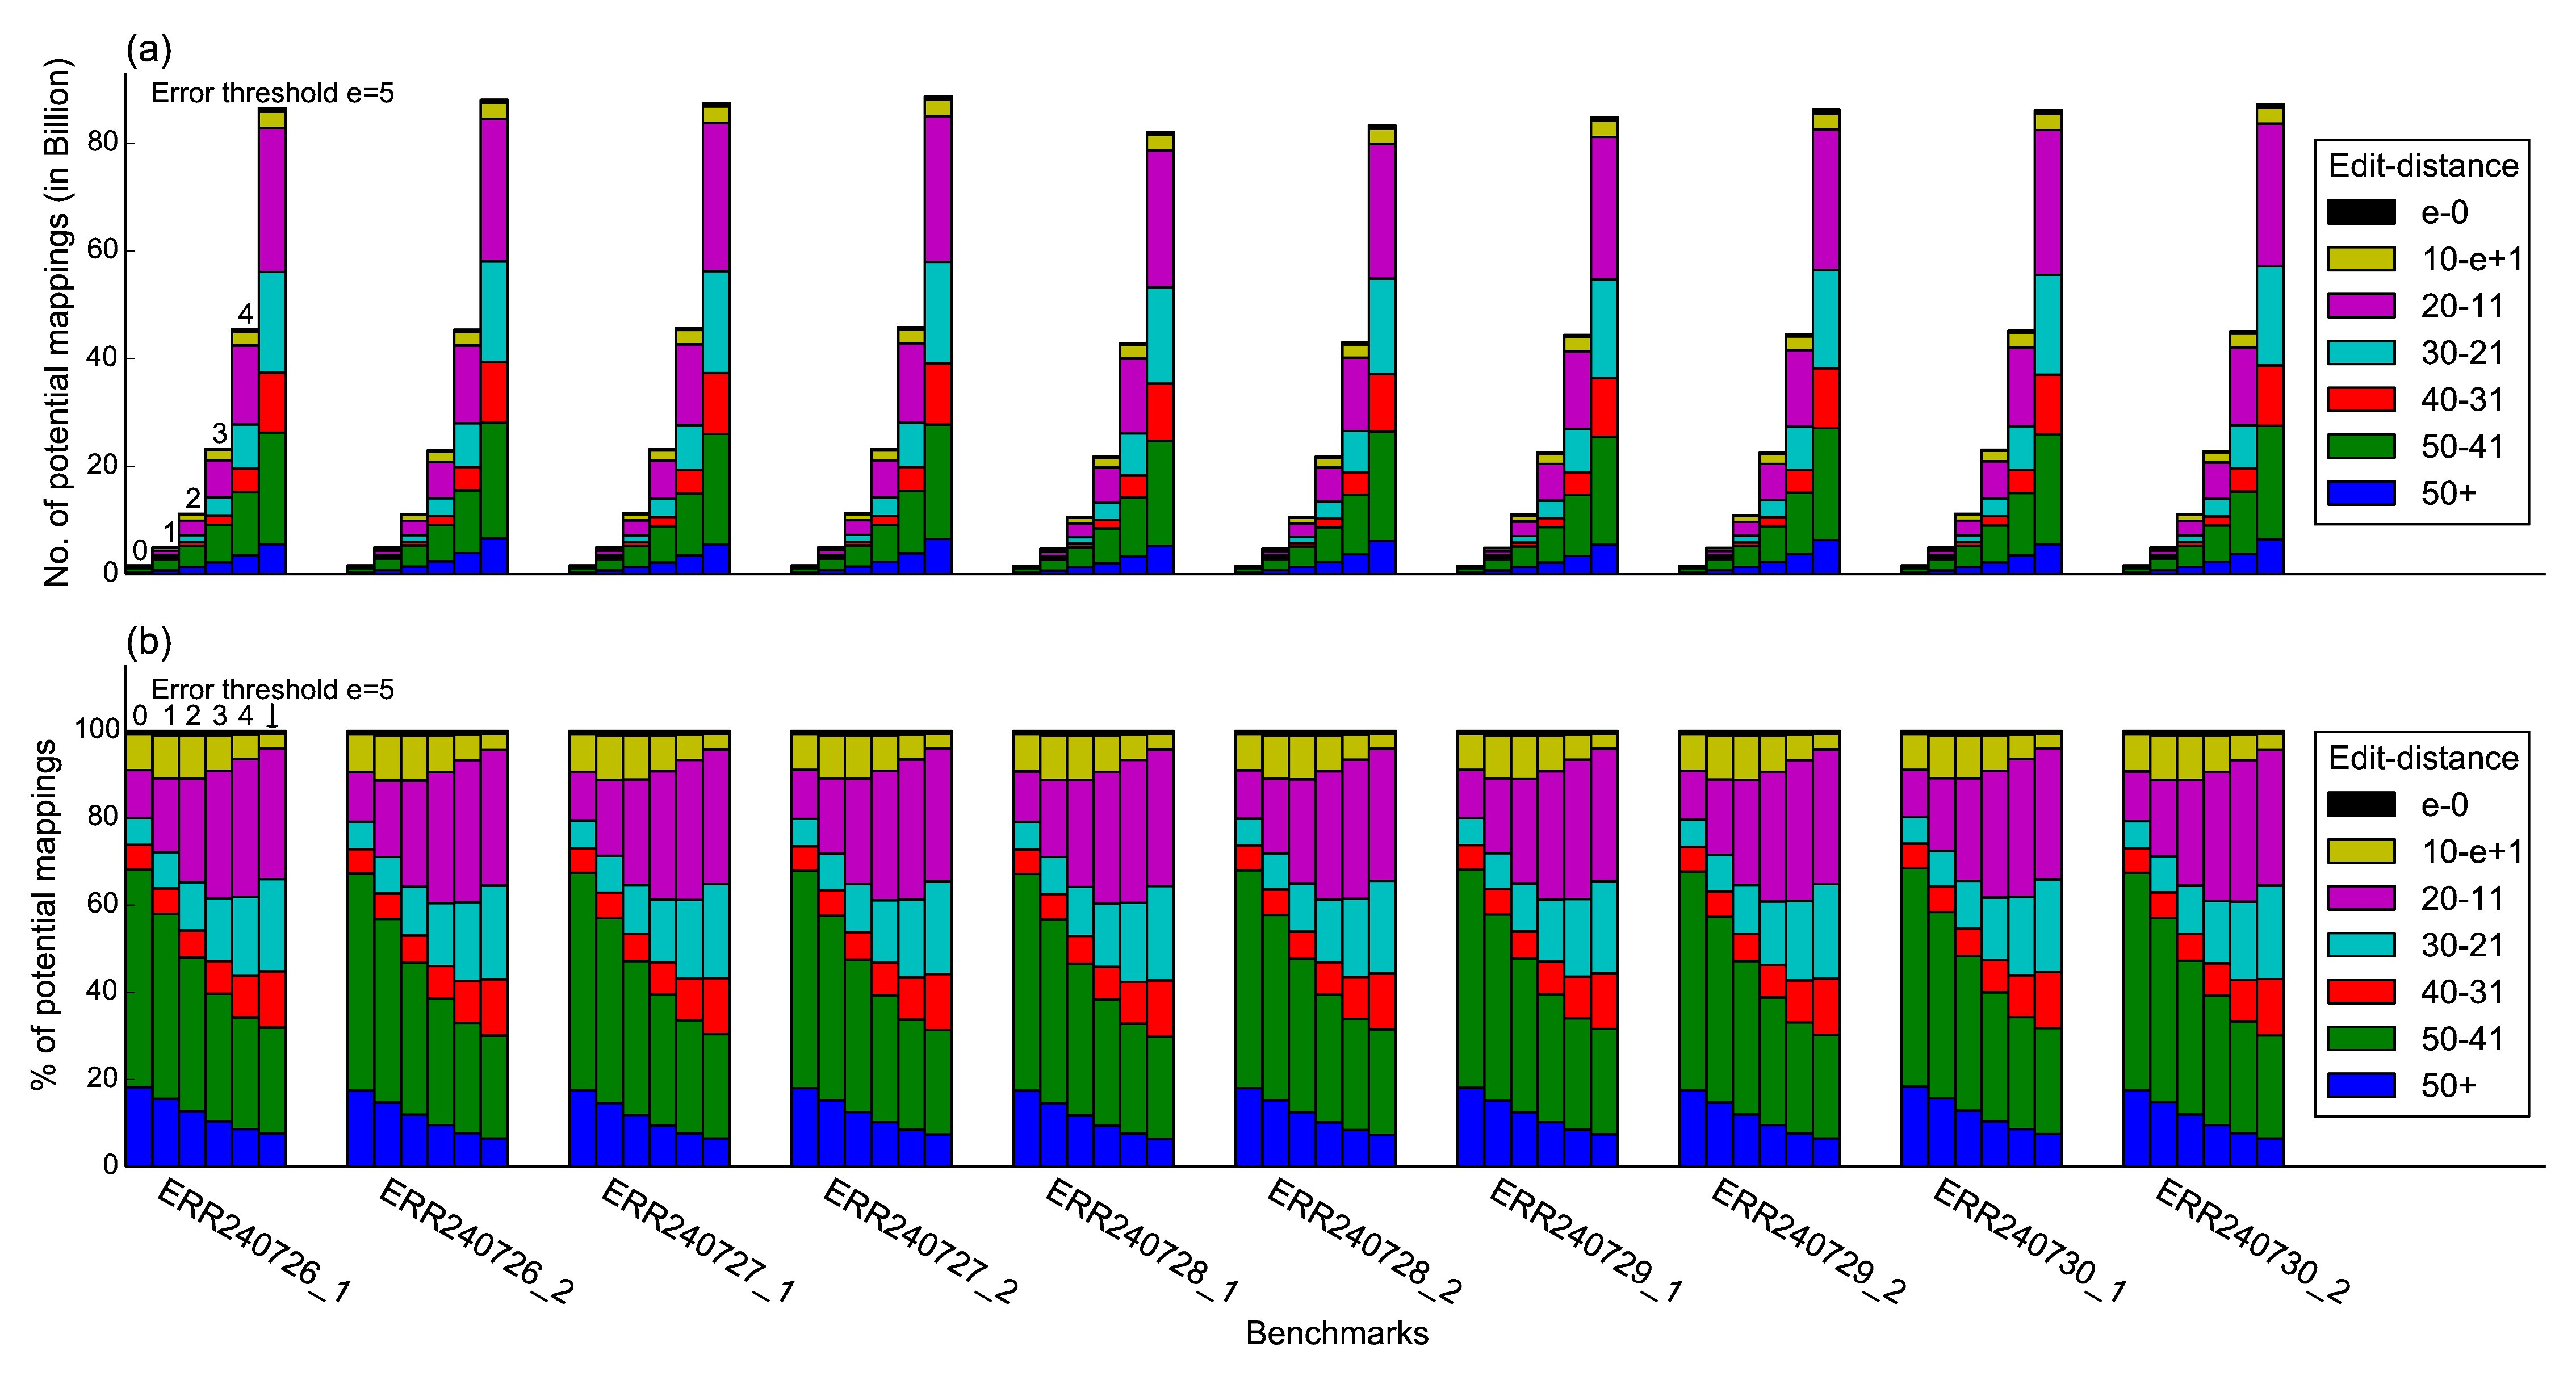
\includegraphics{fig}
\end{figure}
  
  
  
  